\documentclass{scrartcl}
\usepackage[a4paper,margin=2cm,landscape]{geometry}

\usepackage[T1]{fontenc}
\usepackage[utf8]{inputenc}
\usepackage{graphicx}
\usepackage{fancyhdr}
\usepackage{amssymb}

\pagestyle{fancy}
\fancyhf{}
\fancyhead[L]{CS2020/CS4340: guest lecture on executable modelling with Papyrus-RT}
\fancyhead[R]{Handout: turn the robot around}

\newcommand*{\state}[1]{\textit{#1}}

\begin{document}

\begin{center}
  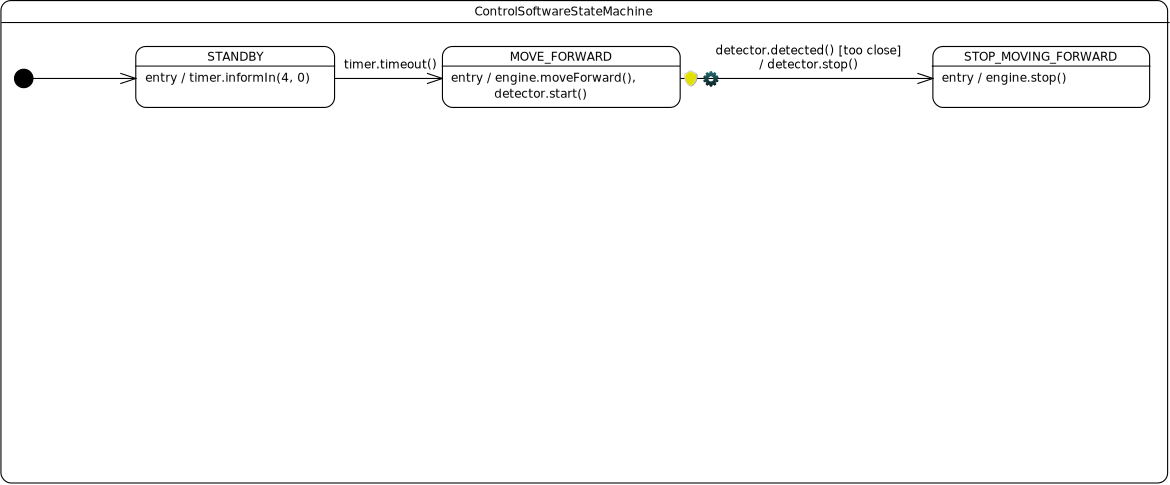
\includegraphics[width=\textwidth]{rover-control-juststop}
\end{center}

\begin{tabular}{l l l}
  \begin{minipage}[t]{.3\textwidth}
    \begin{center}
      \textbf{Engine protocol}
    \end{center}

    You can send:
    \begin{itemize}
    \item moveForward(), moveBackward()
    \item stop()
    \item turnLeft(angle), turnRight(angle)
    \end{itemize}

    You can receive:
    \begin{itemize}
    \item stopped()
    \item turnedLeft(), turnedRight()
    \end{itemize}
  \end{minipage}&
  \begin{minipage}[t]{.3\textwidth}
    \begin{center}
      \textbf{Timer protocol}
    \end{center}

    You can send:
    \begin{itemize}
    \item informIn(secs, nanosecs)
    \end{itemize}

    You can receive:
    \begin{itemize}
    \item timeout()
    \end{itemize}
  \end{minipage}&
  \begin{minipage}[t]{.3\textwidth}
    \begin{center}
      \textbf{Exercise}
    \end{center}

    Add transitions and /entry behaviours to:
    \begin{itemize}
    \item[$\square$] Wait 2 seconds after stopping
    \item[$\square$] Move back for 1 second
    \item[$\square$] Stop for 2 seconds
    \item[$\square$] Turn 138 degrees
    \item[$\square$] Wait two seconds
    \item[$\square$] Return to \state{MOVE\_FORWARDS}
    \end{itemize}
  \end{minipage}\\
\end{tabular}

\end{document}
